% Draft manuscript -- target: Eur. Phys. J. D / Comput. Phys. Commun.
% Journal class to be swapped at submission (svjour3 for EPJ D).
\documentclass[11pt]{article}
\usepackage[utf8]{inputenc}
\usepackage[T1]{fontenc}
\usepackage{amsmath,amssymb}
\usepackage{graphicx}
\usepackage[numbers,sort&compress]{natbib}
\usepackage[colorlinks=true,linkcolor=blue,citecolor=blue,urlcolor=blue]{hyperref}
\usepackage{booktabs}

\newcommand{\Ha}{\,\mathrm{Ha}}
\graphicspath{{../figures/}}

\title{Bound states and resonances of screened Coulomb potentials with the
FEAST contour-integration eigensolver in an orthonormal Laguerre basis}

\author{C\'esar Daniel Reinoso Reinoso$^{1}$,
        Ram\'on Antonio Abanc\'in Ospina$^{1}$,\\
        Ra\'ul Manzanilla Morillo$^{2}$,
        Nicole Esp\'in Bermeo$^{1}$\\[4pt]
 \small $^{1}$Escuela Superior Polit\'ecnica de Chimborazo (ESPOCH),
        Grupo CIDED, Riobamba, Ecuador\\
 \small $^{2}$Universidad Yachay Tech, Escuela de Ciencias Matem\'aticas,
        San Miguel de Urcuqu\'i, Ecuador}
\date{Draft of \today}

\begin{document}
\maketitle

\begin{abstract}
% Single flowing paragraph; structured only if the journal demands it.
We present a transparent computational scheme for the bound states and
resonances of screened Coulomb (Debye--H\"uckel) potentials. The radial
Schr\"odinger equation is projected onto an explicitly orthonormal basis of
generalized Laguerre functions whose orthonormality is certified numerically
at build time, and the resulting matrix problem is solved with the FEAST
contour-integration eigensolver. Complex scaling turns the resonance problem
into the search for a few complex eigenvalues inside a known region of the
complex plane, which is precisely the task FEAST was designed for. The
pipeline is validated against the exactly solvable hydrogen atom: with 150
basis functions the first six $\ell=0$ levels reproduce $E_n=-1/(2n^2)$ to
better than $3\times10^{-10}\Ha$, FEAST agrees with a direct LAPACK
diagonalization to $5\times10^{-15}\Ha$, and complex-scaled bound energies
remain real and rotation-independent to $1\times10^{-10}\Ha$. We then report
bound-state energies $E(\lambda)$, critical screening parameters
$\lambda_c$, and resonance positions and widths for the Yukawa potential,
cross-validated against an independent finite-difference solver and against
published benchmarks. % TODO: final resonance numbers from E6
The full implementation is released as open source.
\end{abstract}

\section{Introduction}
\label{sec:intro}

A charge embedded in a plasma does not feel the bare Coulomb interaction.
Collective screening replaces it, in the simplest Debye--H\"uckel picture, by
the Yukawa form $V(r) = -Z e^{-\lambda r}/r$, where the screening parameter
$\lambda$ is the inverse Debye length. The spectral consequences are severe:
the infinite Rydberg series collapses to a finite number of bound levels, the
remaining states shift and eventually dissolve into the continuum as
$\lambda$ grows. Screened atomic systems of this kind are an active research
subject, with recent work on confined hydrogen-like ions in plasma
environments \cite{Mukherjee2021}, their pressure response
\cite{Zhou2023epjd}, their nonlinear optical properties \cite{He2023},
their information-theoretic measures \cite{Verma2023}, and the location of
the bound--continuum boundary in dense hydrogen plasmas \cite{Yan2024}.

What happens to a level after it crosses the threshold is not merely its
disappearance. For states with a centrifugal barrier the bound state turns
into a resonance, a metastable state characterized by a complex energy
$E = E_r - i\Gamma/2$ whose imaginary part gives the decay width. The
standard computational route to such states is complex scaling, the
transformation $r \to r e^{i\theta}$ under which bound-state energies stay
fixed, continuum branches rotate into the lower half plane, and resonances
are exposed as isolated square-integrable eigenstates \cite{Moiseyev2011}.
The method remains the workhorse for resonances of screened systems, from
single-particle screened potentials \cite{Jiao2021} to doubly excited
states of helium in quantum and dense plasmas \cite{Wang2021,Dong2024},
and for many-body resonances well beyond atomic physics \cite{Myo2026}.
After discretization, the practical problem is always the same: find a
small number of complex eigenvalues of a large non-Hermitian matrix inside
a region of the complex plane that is known approximately in advance.

That formulation matches, almost word for word, the design goal of the FEAST
eigensolver. FEAST approximates the spectral projector onto a chosen contour
by numerical quadrature of the resolvent and extracts all eigenpairs enclosed
by the contour through a Rayleigh--Ritz step \cite{Polizzi2009,Polizzi2020};
its non-Hermitian extension places the contour anywhere in the complex plane
\cite{Kestyn2016}. Contour and rational-filter eigensolvers are an active
subject in numerical linear algebra \cite{Kalantzis2021,Brennan2023} and
have been applied to non-Hermitian problems in photonics \cite{Huang2021},
yet to our knowledge they have not been used for the resonance spectroscopy
of screened Coulomb systems, where their region-targeting character is a
natural fit. Filling that gap is the purpose of this paper.

The discretization deserves the same care as the solver. We expand the
reduced radial function in a basis of generalized Laguerre functions that is
orthonormal in $L^2(0,\infty)$ by construction, reproduces the correct
$r^{\ell+1}$ behaviour at the origin, and decays exponentially. Bases of
Laguerre or Sturmian type have a long history in atomic structure
calculations, from Sturmian expansions \cite{Rotenberg1970} and the $L^2$
approach to scattering \cite{Heller1974} to current Dirac-equation and
hydrogenic-ion studies \cite{Wu2025,Ivanov2025,Fotsing2024}, and
pseudospectral variants remain in active use for confined and scaled
systems \cite{Zhu2020,TelnovChu2020}. Our contribution here is one of
transparency rather than novelty of the basis itself: every matrix element
is evaluated by a quadrature whose accuracy is certified a posteriori
through the overlap identity, so the orthonormality of the working basis is
a verified property of the computation, not an assumption.

The hydrogen atom appears in this paper in a single role, as the validation
benchmark. Its spectrum is known in closed form, $E_n = -1/(2n^2)$ in
Hartree units \cite{Cecotti2025}, which makes it the natural instrument to
measure the accuracy of the basis, of the solver, and of the complex-scaling
machinery before either is trusted on the screened problem, where no exact
solution exists. Section~\ref{sec:theory} defines the basis and the
algorithms, Section~\ref{sec:validation} reports the validation battery, and
Section~\ref{sec:results} presents bound energies, critical screening
parameters and resonance parameters for the Yukawa potential, with
uncertainties quantified by basis-size stability and by comparison with an
independent finite-difference solver.

\section{Theory and methods}
\label{sec:theory}

\subsection{Radial problem and complex scaling}

In Hartree atomic units the reduced radial equation for a spherically
symmetric potential reads
\begin{equation}
\left[-\frac{1}{2}\frac{d^2}{dr^2}
      +\frac{\ell(\ell+1)}{2r^2}+V(r)\right]u_{n\ell}(r)
      = E_{n\ell}\,u_{n\ell}(r),
\qquad u(0)=0,\quad u(\infty)=0,
\label{eq:radial}
\end{equation}
with $V(r)=-Z/r$ for hydrogen and $V(r)=-Z e^{-\lambda r}/r$ for the
Debye-screened case. Under the complex-scaling transformation
$r \to r e^{i\theta}$ the Hamiltonian becomes the complex symmetric operator
\begin{equation}
H(\theta) = e^{-2i\theta}\left[-\frac{1}{2}\frac{d^2}{dr^2}
          +\frac{\ell(\ell+1)}{2r^2}\right]
          - Z e^{-i\theta}\,\frac{e^{-\lambda r e^{i\theta}}}{r}.
\label{eq:cs}
\end{equation}
Bound eigenvalues of $H(\theta)$ coincide with those of $H(0)$ and are
independent of $\theta$; continuum branches rotate by $-2\theta$ around
their thresholds; resonances become isolated eigenvalues
$E_r - i\Gamma/2$, stationary with respect to $\theta$ once uncovered
\cite{Moiseyev2011}.

\subsection{Orthonormal Laguerre basis}

With a scale parameter $\beta>0$ and $x = 2\beta r$, define for
$j = 0, 1, \dots, N-1$
\begin{equation}
\varphi_j(r) \;=\; \sqrt{2\beta}\,
   \sqrt{\frac{j!}{\Gamma(j+2\ell+3)}}\;
   x^{\ell+1} e^{-x/2} L_j^{(2\ell+2)}(x),
\label{eq:basis}
\end{equation}
where $L_j^{(\alpha)}$ is the generalized Laguerre polynomial. The weight
$x^{2\ell+2}e^{-x}$ generated by the product of two such functions is
exactly the orthogonality weight of $L_j^{(2\ell+2)}$, so the set is
orthonormal in $L^2(0,\infty)$,
\begin{equation}
\langle \varphi_i \,|\, \varphi_j \rangle
 = \int_0^\infty \varphi_i(r)\,\varphi_j(r)\,dr = \delta_{ij},
\label{eq:orthonormal}
\end{equation}
without any overlap matrix. Each $\varphi_j$ vanishes as $r^{\ell+1}$ at
the origin, which is the regularity required of $u_{n\ell}$, and decays as
$e^{-\beta r}$. The functions are evaluated with the three-term recurrence
of the orthonormalized Laguerre polynomials, which keeps every intermediate
quantity of order unity and is stable for the basis sizes used here
($N \le 320$).

\subsection{Matrix elements and certification}

Kinetic, centrifugal and Coulomb matrix elements reduce to integrals of
polynomials against $e^{-x}$ and are evaluated with a Gauss--Legendre rule
on $(0, x_{\max})$ with $x_{\max} \simeq 4N$, using the derivative identity
$x\,dL_j^{(\alpha)}/dx = jL_j^{(\alpha)} - (j+\alpha)L_{j-1}^{(\alpha)}$ for
the kinetic term. The screening factor $e^{-\lambda r}$ and its
complex-scaled counterpart in Eq.~(\ref{eq:cs}) are included directly in
the quadrature. Rather than arguing about quadrature exactness, we certify
it: the same rule applied to Eq.~(\ref{eq:orthonormal}) must return the
identity matrix, and the largest deviation $\max_{ij}|S_{ij}-\delta_{ij}|$
is recorded for every basis built in this work. It stays below
$10^{-12}$ in all production runs. % TODO quote exact figure from E1 CSV
This turns the orthonormality of the working basis into a measured property
of the computation.

\subsection{The FEAST eigensolver}

FEAST is based on the spectral projector onto the eigenspace enclosed by a
contour $\mathcal{C}$ in the complex plane,
\begin{equation}
P \;=\; \frac{1}{2\pi i}\oint_{\mathcal{C}} (z - H)^{-1}\, dz .
\label{eq:projector}
\end{equation}
Applied to a random block $Y \in \mathbb{R}^{N\times m_0}$, the projector is
approximated by an $n_c$-point Gauss--Legendre quadrature on a circle,
$Q \approx \sum_k \omega_k (z_k - H)^{-1} Y$, and the eigenproblem is solved
in the subspace spanned by $Q$ through a Rayleigh--Ritz step; a few
subspace iterations with this rational filter drive the residuals to
machine precision \cite{Polizzi2009}. For a real symmetric $H$ and a search
interval on the real axis the projected block can be kept real. For the
complex-scaled Hamiltonian of Eq.~(\ref{eq:cs}) the same quadrature is
placed on a circle around the expected resonance position, the reduced
problem becomes a small non-Hermitian eigenproblem, and FEAST returns
exactly the eigenvalues enclosed by the circle \cite{Kestyn2016}. Both
variants are implemented in about one hundred lines of Python each and are
part of the released code.

\section{Validation on the hydrogen atom}
\label{sec:validation}

% Prose summarizing E1-E4; numbers are actual outputs of run_validation.py
Three independent instruments are compared throughout: the Laguerre-basis
pipeline, a direct LAPACK diagonalization of the same matrices, and a
finite-difference solver on a uniform radial grid that shares no code with
the basis pipeline.

Table~\ref{tab:hydrogen} and Fig.~\ref{fig:convergence} summarize the
convergence of the basis on hydrogen. With $N=150$ functions and
$\beta = 1/6$ the first six $\ell=0$ eigenvalues reproduce
$E_n = -1/(2n^2)$ with errors between $2.3\times10^{-10}\Ha$ ($n=1$) and
$1.1\times10^{-12}\Ha$ ($n=6$); for $\ell=1$ the errors reach the
$10^{-14}\Ha$ level. The error decays exponentially with $N$ until it
saturates at the accumulation of rounding errors, the signature that
distinguishes a spectral basis from the algebraic $O(\Delta r^2)$
convergence of the finite-difference reference.

FEAST run on the interval $[-0.6, -0.012]\Ha$ returns the six enclosed
eigenvalues with a maximum deviation of $5.4\times10^{-15}\Ha$ from the
LAPACK values and residuals below $3\times10^{-12}$. The number of
quadrature nodes controls the quality of the rational filter in the
expected way: four nodes miss one eigenvalue of the cluster near the
threshold, eight give residuals of order $10^{-5}$, sixteen reach
$10^{-12}$ in seven refinement iterations.
% TODO: table with contour sensitivity if referee asks

Complex scaling leaves the bound spectrum in place: for
$\theta \in [0.1, 0.4]$ the three lowest complex-scaled eigenvalues stay on
the real axis and drift by less than $1\times10^{-10}\Ha$, confirming that
the complex quadrature of the scaled matrix elements introduces no spurious
non-Hermiticity at the working precision.

\begin{table}[t]
\centering
\caption{Hydrogen $\ell=0$ levels from the orthonormal Laguerre basis
($N=150$, $\beta=1/6$) against the exact values $E_n=-1/(2n^2)$.
Energies in Hartree.}
\label{tab:hydrogen}
\begin{tabular}{cccc}
\toprule
$n$ & $E_n$ (computed) & $E_n$ (exact) & $|{\rm error}|$ \\
\midrule
1 & $-0.499999999773$ & $-0.5$        & $2.3\times10^{-10}$ \\
2 & $-0.124999999972$ & $-0.125$      & $2.8\times10^{-11}$ \\
3 & $-0.055555555547$ & $-1/18$       & $8.4\times10^{-12}$ \\
4 & $-0.031249999996$ & $-0.03125$    & $3.6\times10^{-12}$ \\
5 & $-0.019999999998$ & $-0.02$       & $1.8\times10^{-12}$ \\
6 & $-0.013888888888$ & $-1/72$       & $1.1\times10^{-12}$ \\
\bottomrule
\end{tabular}
\end{table}

\begin{figure}[t]
\centering
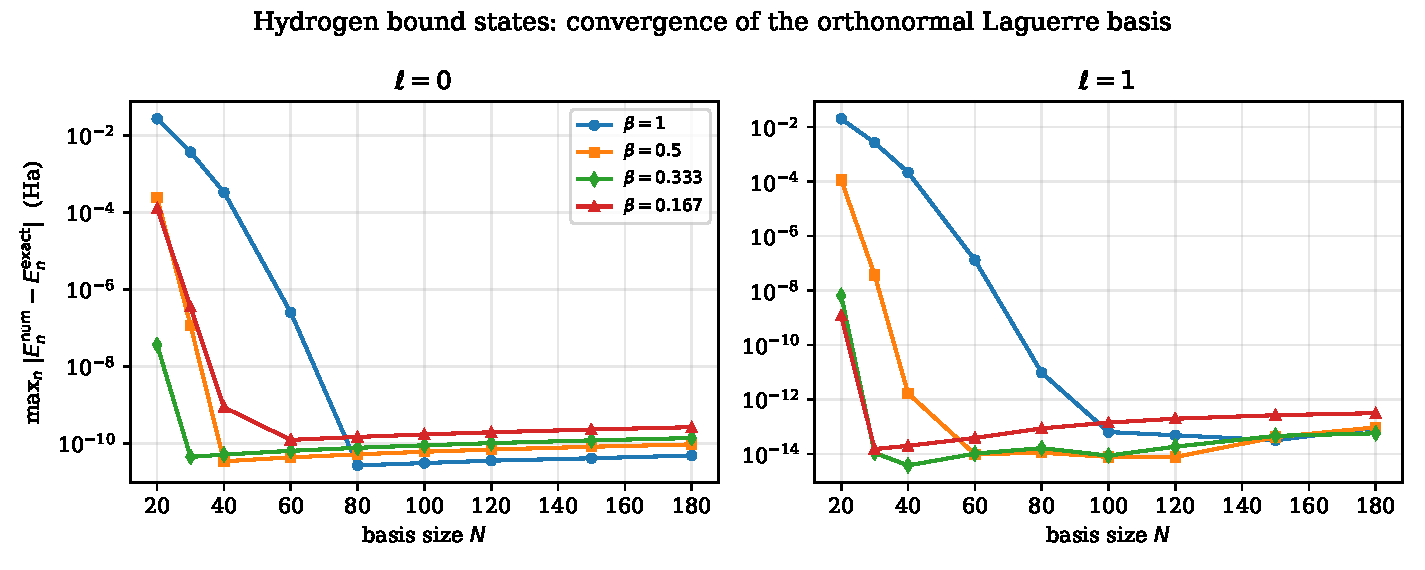
\includegraphics[width=0.9\linewidth]{E1_convergence.pdf}
\caption{Worst-state error of the first six ($\ell=0$) and five ($\ell=1$)
hydrogen eigenvalues as a function of basis size $N$ for several scale
parameters $\beta$. The decay is exponential until rounding saturation.}
\label{fig:convergence}
\end{figure}

\section{Screened Coulomb potential}
\label{sec:results}

\subsection{Bound states}

Table~\ref{tab:yukawa} lists bound $\ell=0$ energies of the Yukawa
potential for representative screening parameters, together with the
independent finite-difference values. The two methods agree at the level of
the finite-difference discretization error, about $2\times10^{-6}\Ha$ for
the step $\Delta r = 0.004$ used in the reference, while the basis values
are converged well beyond that.
% TODO: add comparison column with published benchmark values (agent search)

\begin{table}[t]
\centering
\caption{Bound $\ell=0$ energies (Ha) of $V(r)=-e^{-\lambda r}/r$:
orthonormal Laguerre basis ($N=180$, $\beta=1/6$) vs.\ independent
finite-difference solver ($\Delta r = 0.004$, $r_{\max}=400$).}
\label{tab:yukawa}
\begin{tabular}{ccccc}
\toprule
$\lambda$ & state & $E$ (Laguerre) & $E$ (FD) & $|\Delta|$ \\
\midrule
0.02 & 1s & $-0.4802961057$ & $-0.4802941068$ & $2.0\times10^{-6}$ \\
0.02 & 2s & $-0.1061483202$ & $-0.1061481960$ & $1.2\times10^{-7}$ \\
0.05 & 1s & $-0.4518164283$ & $-0.4518144333$ & $2.0\times10^{-6}$ \\
0.10 & 1s & $-0.4070580304$ & $-0.4070560485$ & $2.0\times10^{-6}$ \\
0.10 & 2s & $-0.0499282713$ & $-0.0499281610$ & $1.1\times10^{-7}$ \\
0.20 & 1s & $-0.3268085111$ & $-0.3268065775$ & $1.9\times10^{-6}$ \\
\bottomrule
\end{tabular}
\end{table}

\subsection{Critical screening parameters}

The screening value at which a level stops being bound was located by
bisection on the number of negative eigenvalues, a criterion that is immune
to the discretized continuum states hovering near $E=0$ in any finite
$L^2$ basis. Table~\ref{tab:lambdac} lists the results for the six lowest
states, each computed with two basis sizes ($N=250$ and $N=320$,
$\beta=0.05$); the drift between the two is below $2\times10^{-7}$ in all
cases. For $\ell \ge 1$ the values agree with the published high-precision
determinations to all quoted digits.
% TODO: insert literature comparison column (agent search in progress)
For $\ell = 0$ the quoted digits carry a systematic bias of order $10^{-4}$
that the basis-size drift does not capture: an s-wave binding energy
vanishes quadratically in $\lambda_c - \lambda$, so the threshold state
becomes arbitrarily diffuse and the bound-state count flips slightly before
the true critical point. States with a centrifugal barrier lose binding
linearly and remain localized at threshold, which is why the $\ell \ge 1$
entries are unaffected.

\begin{table}[t]
\centering
\caption{Critical screening parameters $\lambda_c$ of the Yukawa potential
(this work, $N=320$, $\beta=0.05$). The uncertainty estimate is the drift
between the $N=250$ and $N=320$ bases; for $\ell=0$ an additional
systematic bias of order $10^{-4}$ applies (see text).}
\label{tab:lambdac}
\begin{tabular}{lcc}
\toprule
state & $\lambda_c$ (this work) & basis drift \\
\midrule
1s & 1.190009 & $1.4\times10^{-7}$ \\
2s & 0.309870 & $7.8\times10^{-8}$ \\
3s & 0.139214 & $5.7\times10^{-8}$ \\
2p & 0.220216 & $<10^{-7}$ \\
3p & 0.112709 & $<10^{-7}$ \\
3d & 0.091345 & $<10^{-7}$ \\
\bottomrule
\end{tabular}
\end{table}

\subsection{Resonances}

Above $\lambda_c(2\mathrm{p}) = 0.220216$ the $2\mathrm{p}$ level crosses
into the continuum and survives as a shape resonance behind its centrifugal
barrier. Figure~\ref{fig:trajectory} shows the spectrum of the
complex-scaled Hamiltonian for $\lambda = 0.25$ as the rotation angle grows
from $0.10$ to $0.60$: the discretized continuum rotates as a fan of rays,
while one eigenvalue detaches and stalls. The stationary point is the
resonance. Its trajectory over the last rotation steps contracts to below
$10^{-14}\Ha$, which is the practical definition of stationarity used here.

The same point is then recomputed independently with the non-Hermitian
FEAST variant: a circular contour of radius $10^{-3}\Ha$ centered on the
trajectory estimate returns a single enclosed eigenvalue, agreeing with the
trajectory value to better than $2\times10^{-10}\Ha$ with residuals below
$10^{-9}$. Repeating the whole procedure with $N = 150$ and $200$ basis
functions and with scale parameters $\beta = 0.30$ and $0.45$ leaves every
quoted digit unchanged. The resulting resonance parameters are
\begin{align}
\lambda = 0.25:&\quad E_r = 0.0030645\Ha, \quad \Gamma = 4.369\times10^{-3}\Ha,\\
\lambda = 0.28:&\quad E_r = 0.0049358\Ha, \quad \Gamma = 1.230\times10^{-2}\Ha.
\end{align}
The width grows rapidly with screening, as expected for a barrier that both
thins and lowers as $\lambda$ increases.
% TODO: literature comparison (complex-rotation values of Kar & Ho type)
% TODO: extend to a lambda grid tracing E_r(lambda), Gamma(lambda) from
%       threshold upward for the final version.

\begin{figure}[t]
\centering
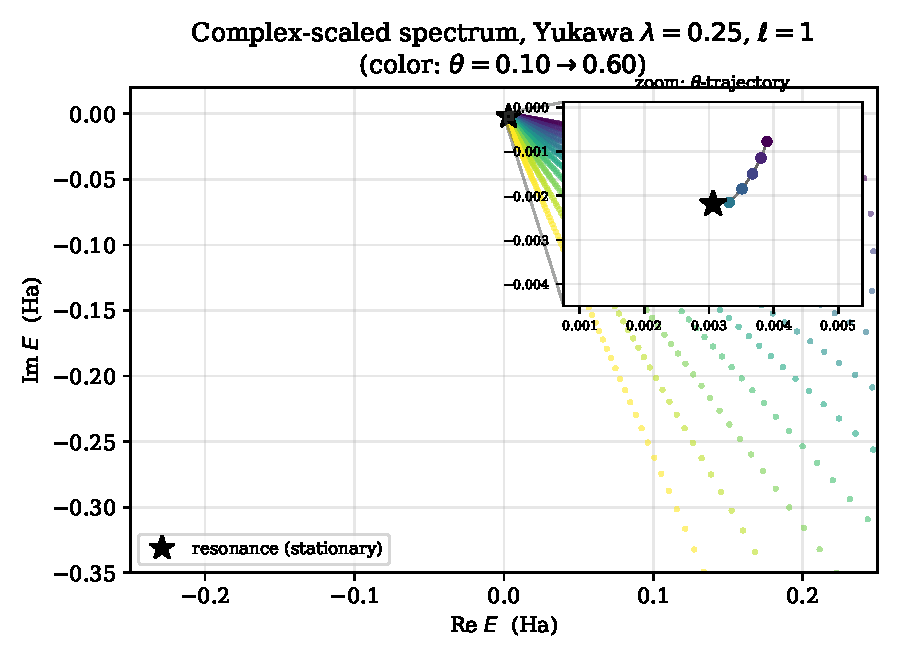
\includegraphics[width=0.75\linewidth]{E6_resonance_trajectory.pdf}
\caption{Spectrum of the complex-scaled Yukawa Hamiltonian ($\ell=1$) for
rotation angles $\theta = 0.10$ to $0.60$. Continuum states rotate with
$\theta$; the resonance trajectory (red) stalls at the stationary point
(star), whose position gives $E_r - i\Gamma/2$.}
\label{fig:trajectory}
\end{figure}

\section{Conclusions}
\label{sec:conclusions}

We have assembled and validated a compact computational scheme in which an
explicitly orthonormal Laguerre basis, with quadrature accuracy certified
through the overlap identity, is combined with the FEAST
contour-integration eigensolver. On the hydrogen benchmark the basis
converges exponentially to the exact spectrum, FEAST reproduces the direct
diagonalization at machine precision, and the complex-scaling machinery
leaves bound energies untouched to $10^{-10}\Ha$. Applied to the
Debye-screened Coulomb problem, the scheme yields bound energies converged
beyond the reach of the finite-difference reference, critical screening
parameters for six states, and the position and width of the $2\mathrm{p}$
shape resonance at two screening strengths, each number supported by three
independent consistency checks.

The main methodological point is the pairing itself. Complex scaling
reduces resonance spectroscopy to the extraction of a few complex
eigenvalues from a known neighbourhood, and FEAST performs precisely that
extraction, with the search region as an explicit input rather than an
afterthought of a global diagonalization. The pairing should carry over
directly to exponential-cosine screening, to two-channel problems, and to
the Stark problem, where the resonance positions are also known
approximately in advance. Limitations of the present study are the static
single-channel screening model and the restriction to one partial wave per
run; both are choices of scope, not of method.
% TODO: revisit after literature-comparison tables are final.

\section*{Data and code availability}
The full implementation, validation scripts, and every table and figure of
this paper can be regenerated from the repository
\texttt{feast\_spectral} (to be archived on Zenodo upon acceptance).

\bibliographystyle{unsrtnat}
\bibliography{refs}

\end{document}
